\section{Durchführung}
\label{sec:Durchfuehrung}
In diesem Kapitel sollen die einzelnen Schritte des Versuches erklärt werden.
\subsection{Aufbau}
\label{sec:aufbau}
Der Aufbau ist Schematisch in \autoref{fig:versuchsaufbau} zu erkennen, ein Foto des realen Aufbaus ist in 
\autoref{fig:realaufbau} zu sehen. Als Lichtquelle wird eine Halogenlampe
genutzt. Ihr Licht wird mithilfe des Kondensors durch eine Lichtzerhacker auf ein aus Kalkspaat bestehendes Glan-Thompson-Prisma abgebildet.
Das Prisma ist mit einem Geniometer verbunden sodass esin verschiedenen Winkeln $\theta_1$ und $\theta_2$ eingestellt
werden kann und diese Winkel auch abgelesen werden können. Nach durlauf des Prismas ist das Licht linear 
polarisiert und läuft durch eine Bohrung im ersten Polschuh des Elektromagneten in eine im Luftspalt zwischen 
den Polschuhen platzierten Probe ein. Anschließend läuft es auf gleiche Weise durch eine Bohrung im zweiten Polschuh
wieder aus dem B-Feld aus. Nun wird das Licht durch einen Interferenzfilter geleitet mit welchem einzeln
Wellenlängen ausgewählt werden können. Der Filter lässt sich austauschen, so können unterschiedliche Wellenlängen
untersucht werden. Anschliesend trifft das nun monochromatische Licht auf ein zweites Glan-Thompson-Prisma
wo der Lichtstrahl in zwei senkrecht zueinander polarisierte Lichtstrahlen aufgeteilt wird. Diese durchlaufen dann
jeweils eine Sammellinse und werden mit dieser auf je einen Bleisulfit Photowiderstand abgebildet. Die beiden
Photowiderstände sind mit einem Differenzenverstärker verbunden dessen Ausgangssignal wiederum in einen 
Selektivverstärker geleitet wird. Das Ausgangssignal des Selektivverstärkers wird dann mit einem Oszilloskop
gemessen. Der Differenzenverstärker verstärkt die Spannungsdifferenz zwischen den Photowiderständen, wenn also 
beide Lichtsrahlen die aus dem zweiten Glan-Thompson-Prisma austreten die gleiche Intensität haben ist das 
Ausgangssignal gleich null. Der Selektivverstärker muss auf die gleiche Frequenz eingestellt werden wie 
der Lichtzerhacker, so wird ein rauschen der Photowiderstände unterdrückt. Der Elektromagnet wird von einem 
Konstantstromgerät gespeist, so ist die magnetische Flussdichte über die Stromstärke $I$ einstellbar.

\begin{figure}
    \centering
    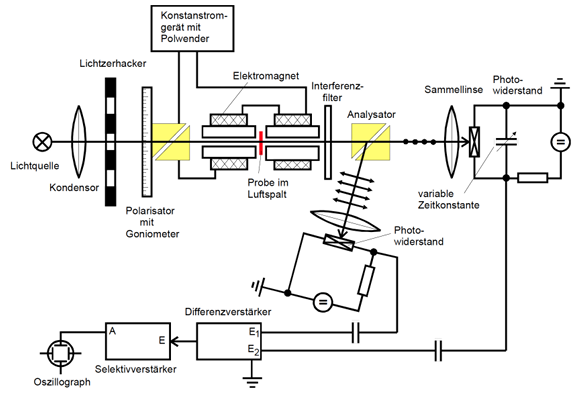
\includegraphics[width=1\textwidth]{content/grafiken/versuchsaufbau.JPG}
    \caption{Der Schematische Versuchsaufbau. [1]}
    \label{fig:versuchsaufbau}
  \end{figure}

  \begin{figure}
    \centering
    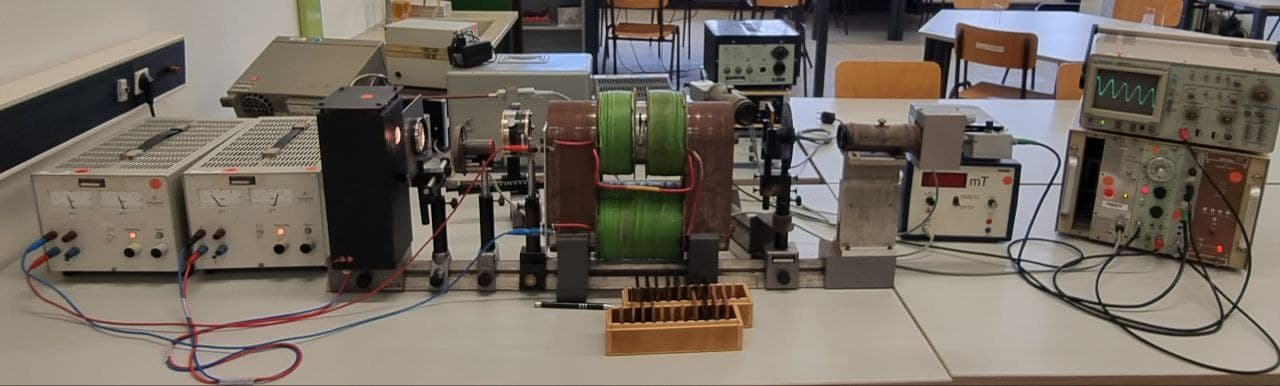
\includegraphics[width=1\textwidth]{content/grafiken/realer versuchsaufbau.JPG}
    \caption{Der tatsächliche Versuchsaufbau im Labor.}
    \label{fig:realaufbau}
  \end{figure}

\subsection{Justierung der Messapparatur}
\label{sec:justierung}
Um die Messapparatur zu justieren wird das sichtbare Spektrum der Halogenlampe genutzt. 
Die Probe und der Interferenzfilter werden noch nicht eingesetzt. Es wird zunächst eine
scharfe Abbildung auf dem ersten Prisma erzeugt. Dann wird durch das für den ordentlichen
Strahl voregsehene Austrittsfenster des zweiten Prismas geschaut. Der Strahl muss durch
drehung des ersten Prismas zum verschwinden gebracht werden können. Ist dies nicht der
Fall muss das zweite Prisma noch um seine vertikale Achse ausgerichtet werden. Der Strahl 
sollte auf beide Prismen senkrecht auftreffen. Anschließend muss überprüft werden ob das 
Licht durch die Sammellinsen auf die Photowiderstände trifft. Im Optimalfall kann das Licht 
durch drehung des ersten Prismas zwischen den beiden Photowiderständen hin und her geschaltet werden.
Wenn das der Fall ist wird der Lichtzerhacker auf eine Frequenz von $f=\SI[]{450}[]{\hertz}$ eingestellt.
Die Mittenfrequenz des Selektivverstärkers wird auf den gleichen Wert eingestellt. Die Güte des 
Selektivverstärkers wird auf den Maximalwert $Q=100$ eingestellt um einen möglichst schmalen verstärkten
Frequenzbereich zu erreichen. Die Mittenfrequenz wird mithilfe des Oszilloskops noch nachgeregelt um
einen Maximalausschlag zu erreichen. 

\subsection{Versuchsdurchführung}
\label{sec:versuchsdurchfuehrung}
Zunächst wird die magnetische Flussdichte $B$ bestimmt. Dazu wird das Konstantstromgerät auf den Höchststrom
von $I=\SI[]{10}[]{\ampere}$ eingestellt und eine Hallsonde durch ein Loch in den Polschuhen geschoben. Nun wird 
abhängig von der Position der Sonde die Fussdichte gemessen und notiert. Nun werden nacheinander drei GaAs-
(Galliumarsenit-) Proben, eine hochreine, eine schwach und eine stark n-dotierte, im Luftspalt zwischen den
Polschuhen platziert und jewils der Winkel $\theta$ der Faradayrotation für 9 verschiedene Wellenlängen, also 
mit 9 verschiedenen Polarisationsfiltern gemessen. Dazu wird das erste Prisma so um seine Längsachse rotiert das 
sich am Oszilloskop möglichst keine Spannung mehr ablesen lässt. Die Winkeleinstellung wird vom
Goniometer abgelesen und als $\theta_1$ notiert. Dann wird das B-Feld langsam heruntergeregelt und umgepolt.
Das Prisma wird erneut so rotiert das sich auf dem Oszilloskop möglichst kein Ausschlag mehr erkennen lässt.
Der zweite Winkel wird als $\theta_2$ notiert. Der Winkel $\theta$ ergibt sich dann über:
\begin{equation}
  \label{eq:theta}
  \theta=\frac{1}{2}(\theta_2-\theta_1)
\end{equation} 